\documentclass{article}
\usepackage[submission]{colm2026_conference}

\usepackage{microtype}
\usepackage{graphicx}
\usepackage{hyperref}
\usepackage{url}
\usepackage{booktabs}
\usepackage{multirow}
\usepackage{lineno}
\usepackage{amsmath}
\usepackage{amssymb}
\usepackage{tikz}
\usetikzlibrary{arrows.meta,positioning,calc}

\input{math_commands.tex}

\definecolor{boxblue}{RGB}{0,114,178}
\definecolor{pastein}{RGB}{213,94,0}
\definecolor{timegray}{RGB}{80,80,80}
\definecolor{darkblue}{rgb}{0, 0, 0.5}
\hypersetup{colorlinks=true, citecolor=darkblue, linkcolor=darkblue, urlcolor=darkblue}


\title{Noising Prompts in Continuous Diffusion Language Models for Conditional Generation}

% Authors must not appear in the submitted version (handled by the "submission" option).
\author{Anonymous}

\begin{document}

\ifcolmsubmission
\linenumbers
\fi

\maketitle

\begin{abstract}
We revisit a standard accepted practice in the continuous diffusion language model
literature of fixing conditioning prompt tokens clean during training.
Rather, we make a very simple modification: also noise the conditioning prompt tokens during training.
We demonstrate that under this modified training objective, we achieve better generalization 
in combinatorial reasoning tasks such as Sudoku and N-Queens, with significant improvements on harder
variants ($1.25\% \to 25.45\%$ solve rate on Sudoku Hard). Moreover, our models exhibit higher generation
diversity. Our method can be seen as a generalization of classifier-free guidance training. 

% TODO: ~150 words. Core claim: standard conditional continuous-diffusion LMs hold
% conditioning (clue) tokens clean throughout corruption ("paste-in"). We instead noise
% the conditioning tokens during training, controlled by p_condclean (prob a conditioning
% token is kept clean). Lower p_condclean (more noising) consistently improves infill
% accuracy and, especially, solution COVERAGE on Sudoku (easy) and N-Queens (8x8, 10x10).
% Headline numbers: Sudoku-easy N=10k acc 87.55% (p=0.2) vs 51.45% (p=1.0);
% N-Queens accuracy AND coverage monotonic across all settings. Position as generalization of CFG.
\end{abstract}

\section{Introduction}
\label{sec:intro}
% TODO: Motivate conditional generation in continuous diffusion LMs (infilling puzzles:
%   observe clue cells, generate the rest). Standard practice: clamp conditioning tokens
%   clean at every denoising step ("paste-in" / always-clean clues, our p_condclean=1.0).
% TODO: State the surprising finding: NOISING conditioning tokens during training improves
%   conditional generation; clean-clue training collapses toward fewer modes.
% TODO: Frame as a generalization of classifier-free guidance (p=1 conditional-only,
%   p=0 unconditional-only). See notes June 11-12.
% TODO: Contributions bullet list (the noised-conditioning training scheme; cross-task
%   evidence on Sudoku + N-Queens; coverage as the discriminating metric).
% Citation needs: \cite{TODO-CFG}, \cite{TODO-FLM}, \cite{TODO-diffusion-forcing}.


Fundamentally, diffusion and flow models learn a score or velocity corresponding to an ODE
which can be integrated to transform a base distribution to the target data distribution.
Their objective can be parameterized in different ways,
including the denoising parametrization $\hat{x}_1(x_t)$, where the goal is to predict a
clean target data $x_1$ given a current noisy input $x_t$.

Our framework is to view this denoising learning objective from the lens of conditional prediction:
given a noisy input, predict a clean target. We then see the varying levels of noise
corruption of the input as a form of curriculum learning, where the model is trained on
harder (more noisy) inputs and easier (less noisy) inputs.

In practice for language modelling, conditional generation is the main paradigm: given a
conditioning prompt, generate a response. Currently, conditional generation in continuous
diffusion language models and flow language models utilize the following learning objective: given
conditioning tokens $x^c$ and a noised response $y_t$, predict the target response $y_1$.
Likewise in sampling, the conditioning tokens are fixed and non-noised. 

We improve this conditional learning objective
by allowing conditional tokens to also be noised, where the model is given
a noised conditional input $x_t^c$ along with the current noised response $y_t$. We see this modification
as extended curriculum learning, where the prediction problem $(x, y_t) \to y$ is made more difficult not
just by increasing the amount of noise in the current response input $y_t$ but also by
increasing the amount of noise in the conditioning input. Moreover, by noising the conditioning input,
our model has a wider target that it can learn from
(also needs to predict the denoised conditioning input), making learning more compute
efficient. Varying the level of noise
on the conditioning input can be seen as a generalization of classifier-free guidance training.
Empirically, we verify on various reasoning and generalization tasks, such as Sudoku and N-Queens. We find that
by additionally noising the conditioning inputs, we get better generalization on these reasoning benchmarks
and exhibit higher levels of generation diversity.

\begin{figure}[t]
\centering
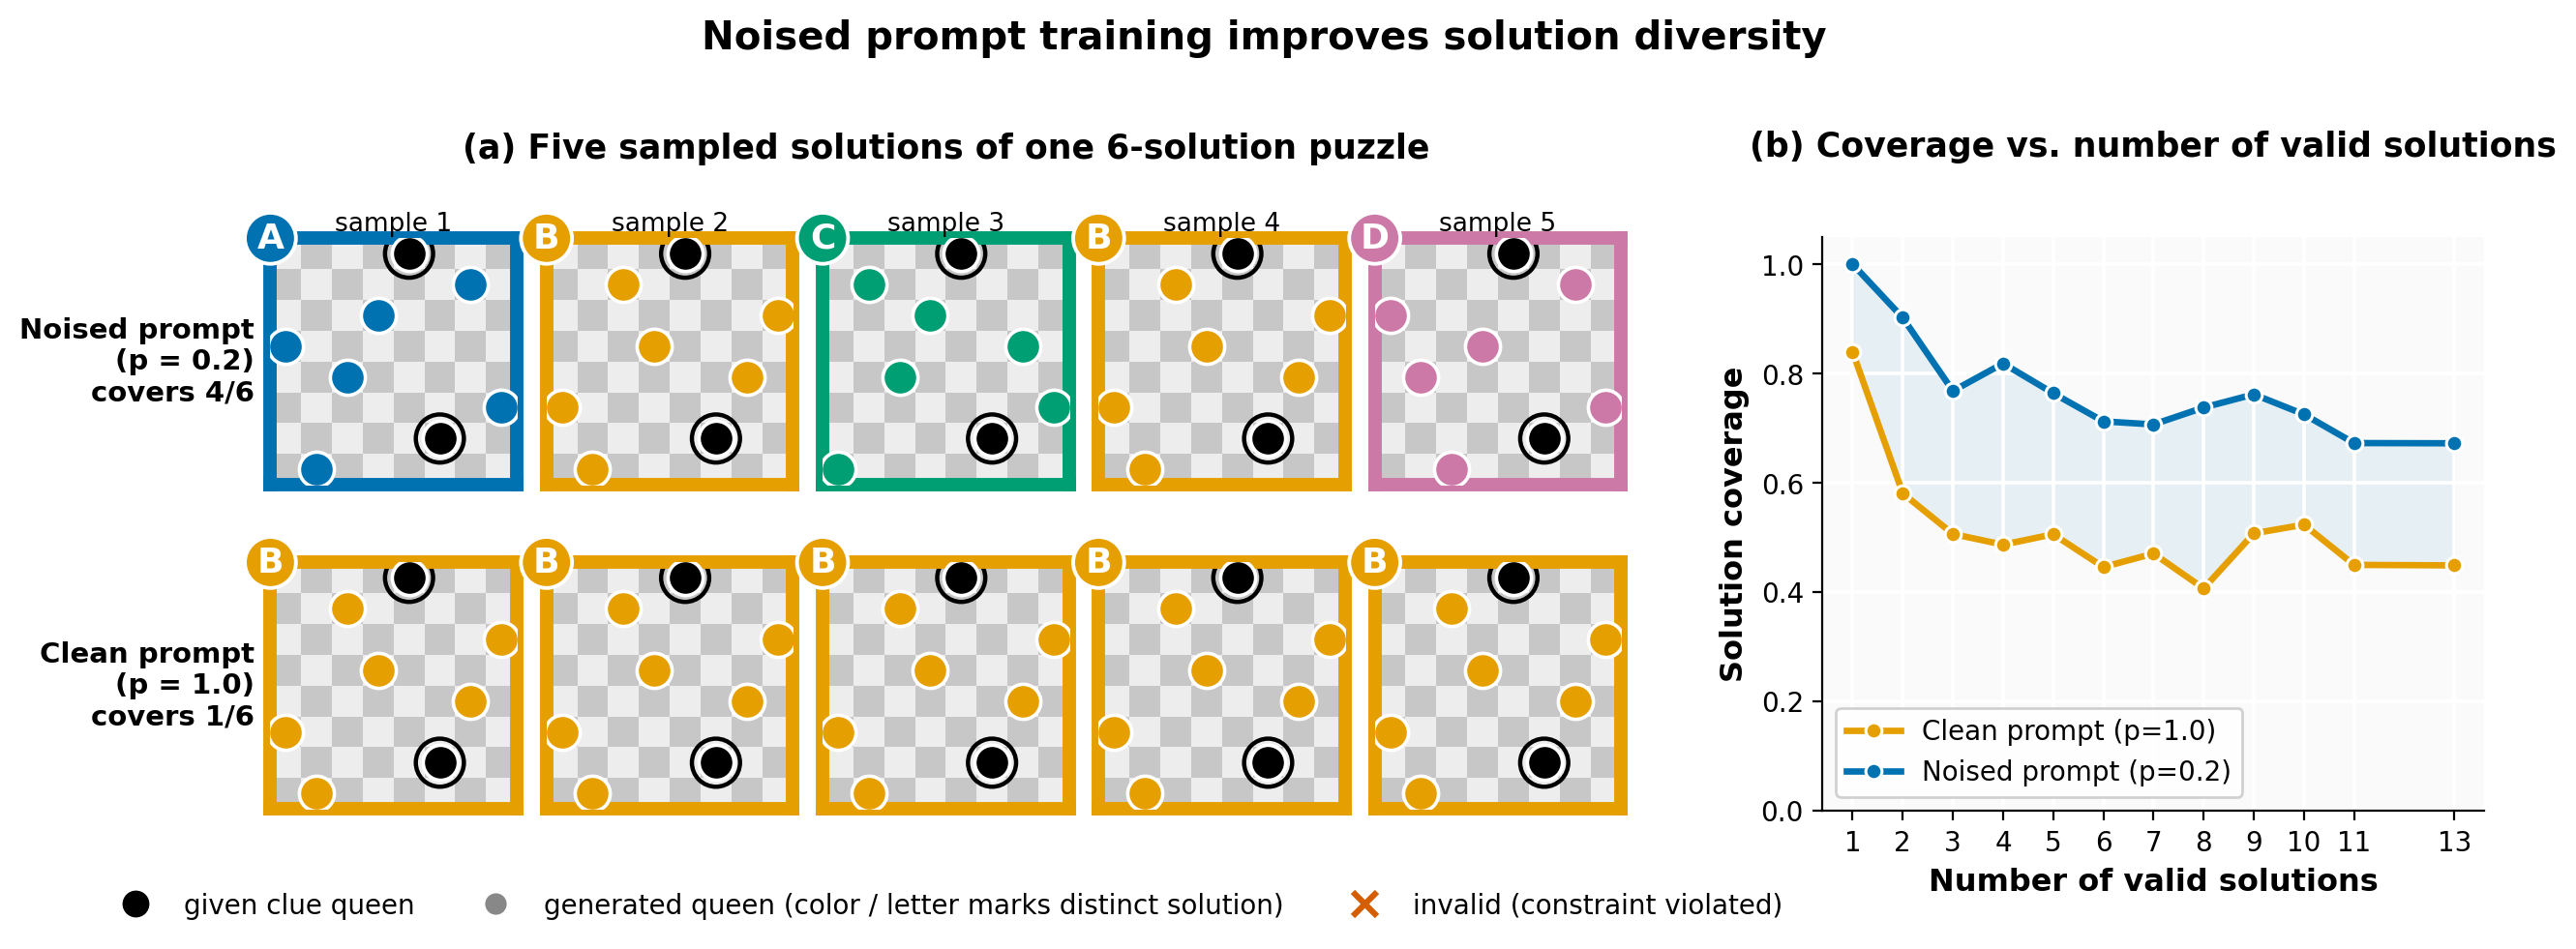
\includegraphics[width=\linewidth]{figures/nqueens_combined.png}
\caption{\textbf{Noising the conditioning tokens improves solution diversity.} \emph{(a)} Five board generations of a single held-out N-Queens ($8\times8$)
puzzle that admits six distinct valid solutions (distinguished by color and letter). A model trained with noised conditioning tokens ($p_\text{condclean}{=}0.2$, top) spreads its
generations across the solution set ($4/6$ distinct solutions), whereas the standard ``paste-in''
model that keeps conditioning tokens clean throughout training ($p_\text{condclean}{=}1.0$, bottom) mode-collapses
onto a single completion ($1/6$). \emph{(b)} Solution coverage as a function of the number of valid
solutions admitted by the input board, over $750$ held-out $10\times10$ puzzles with $k{=}20$
generations each. The noised-prompt model dominates the clean-prompt model at every
solution count. We quantify this gap in Section~\ref{sec:nqueens}.}
\label{fig:teaser}
\end{figure}


\section{Background and Related Work}
\label{sec:background}

\paragraph{Diffusion and flow generative models.}
Denoising diffusion and score-based models generate data by gradually corrupting samples toward a
simple base distribution and learning to reverse this process~\citep{ddpm, song2021sde}. Flow
matching and stochastic interpolants~\citep{lipman2023flow, albergo2023interpolants} give a closely
related and more general view: a time-dependent interpolation between the base and data distributions
defines a velocity field whose ordinary differential equation (ODE) transports noise to data, with
diffusion as a special case. The learning target admits several equivalent
parameterizations---predicting the injected noise, the velocity, the score, or directly the clean
datapoint $x_1$ from a noised input $x_t$ ($x_1$-prediction). We work throughout in the
flow and $x_1$-prediction setting.

\paragraph{Diffusion and flow language models.}
Applying these models to text is complicated by the discreteness of tokens. One line of work operates
directly in discrete state spaces, defining absorbing or uniform corruption processes over tokens:
D3PM~\citep{d3pm}, score-entropy discrete diffusion (SEDD)~\citep{sedd}, masked diffusion language
models (MDLM)~\citep{mdlm}, and large-scale masked diffusion LMs such as LLaDA~\citep{llada}. 
A second line embeds tokens into a continuous space, running continuous gaussian diffusion over those
representations, and converting back to tokens: Diffusion-LM~\citep{diffusion_lm}, DiffuSeq~\citep{diffuseq},
and CDCD~\citep{cdcd}. Recent work operates specifically on one-hot vectors on the probability simplex or 
on learned / pre-trained embeddings: Flow Map Language
Models~\citep{flm}, Discrete Flow Maps~\citep{discrete_flow_maps}, hyperspherical
flows~\citep{hyperspherical_flows}, and embedded language flows (ELF)~\citep{elf}. Our work builds on
this continuous-flow family and adopts its standard denoising ($x_1$-prediction) objective. By default,
these models do conditional generation by holding conditioning tokens clean throughout training
and moreover during sampling, where conditioning tokens are re-pasted at every sampling step ~\citep{flm, elf}.
We term this default method as \emph{paste-in} conditioning.

Diffusion forcing~\citep{diffusion_forcing} and AR-Diffusion ~\citep{ar_diffusion} assign per-token noise levels rather 
than a single shared noise level for the entire sequence. This framework
motivates the notion of multiple noise levels across the sequence, where conditioning tokens may
carry a different noise level than response tokens.


\paragraph{Classifier-free guidance.}
Classifier-free guidance~\citep{cfg} jointly trains a conditional and an unconditional model by
randomly dropping the conditioning signal, then combines their predictions at sampling time to trade
off fidelity against diversity. The amount of conditioning signal in the sequence is binary:
it is either fully injected or fully discarded. Our method can be seen as a continuous generalization
of CFG training: the amount of conditioning signal can be smoothly interpolated by the amount of noise 
(parametrized by time $t \in [0,1]$),
where the end points zero noise  ($t = 1$) and full noise ($t = 0$) recovers the binary CFG inclusion/exclusion.


\paragraph{Corrupting conditioning / prefix tokens.}
Corrupting the conditioning information during training has appeared in several
settings, though rarely for language. In image generation, cascaded diffusion
models~\citep{cascaded} apply conditioning augmentation, deliberately adding noise to the
low-resolution conditioning image fed to each super-resolution stage; this improves robustness to artifacts produced by upstream
stages. Classifier-free guidance~\citep{cfg} can likewise be seen as the extreme case of corrupting the conditioning by
removing it entirely. For language, corrupting the conditioning is far less explored and the evidence
is mixed. Blockwise SFT for diffusion language models~\citep{blockwise_sft} reports that model performance
degrades as the amount of noise on noisy prefixes increases,
and so explicitly freezes the prefix clean.

Most directly related, prompt infilling work for masked diffusion language
models~\citep{prompt_infill} unlocks prompt infilling by masking the prompt as well as the response
during training, rather than masking the response alone. ~\citep{prompt_infill} generate 
multiple prompts and select the best one, offering an alternative to prompt engineering.
In contrast, our method noises conditioning tokens in \emph{continuous} diffusion models during training 
across a continuum of corruption levels, which can be seen as an expanded curriculum objective.
Moreover, there are no changes to inference; the inference-time conditioning
tokens are kept clean and no further additional generation or scoring is necessary.  

\paragraph{Combinatorial reasoning and generalization benchmarks.}
We evaluate on Sudoku and N-Queens, constraint-satisfaction tasks where solving unseen instances
requires learning the underlying rules rather than memorizing input/output pairs. Both have been used
measure to reasoning and moreover generalization ability in recursive and generative reasoning models~\citep{trm, gram}.
In particular, N-Queens admits many valid solutions per board, which lets us measure not only accuracy but also
the diversity of generated solutions, following 
GRAM~\citep{gram}.

\section{Method}
\label{sec:method}

\begin{figure}[t]
  \centering
  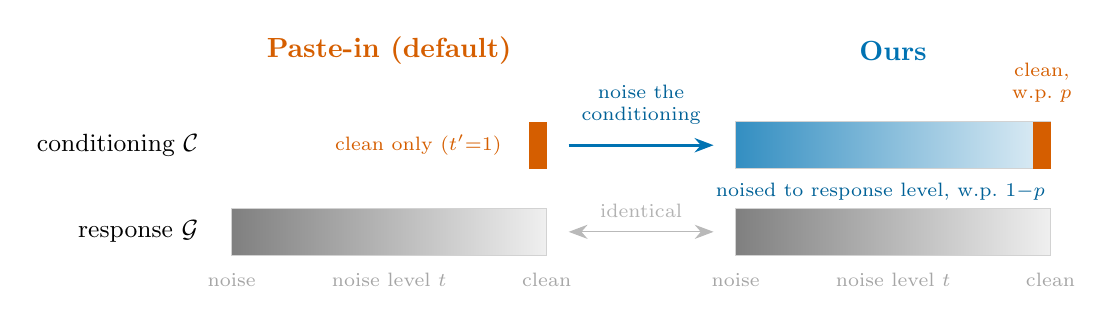
\begin{tikzpicture}[font=\small, >={Stealth[length=2.4mm]}]
  \def\W{4.0}\def\h{0.30}
  \def\yc{1.25}\def\yr{0.15}
  \def\Lx{0}\def\Rx{6.4}
  
  % (no full-range tracks: paste-in conditioning must read as a near-zero-width point)
  
  % ===== LEFT panel: paste-in =====
  % conditioning: ONLY a thin clean sliver at t'=1 (same orange cap as Ours) -> tiny measure
  \fill[pastein] (\Lx+\W-0.22,\yc-\h) rectangle (\Lx+\W,\yc+\h);
  \node[pastein,font=\scriptsize,anchor=east] at (\Lx+\W-0.45,\yc) {clean only ($t'{=}1$)};
  \shade[left color=black!50,right color=black!6] (\Lx,\yr-\h) rectangle (\Lx+\W,\yr+\h);
  \draw[gray!35] (\Lx,\yr-\h) rectangle (\Lx+\W,\yr+\h);
  
  % ===== RIGHT panel: ours =====
  \shade[left color=boxblue!80,right color=boxblue!12] (\Rx,\yc-\h) rectangle (\Rx+\W,\yc+\h);
  \draw[gray!35] (\Rx,\yc-\h) rectangle (\Rx+\W,\yc+\h);
  \fill[pastein] (\Rx+\W-0.22,\yc-\h) rectangle (\Rx+\W,\yc+\h);
  \node[pastein,font=\scriptsize,anchor=south,align=center] at (\Rx+\W-0.11,\yc+\h+0.12) {clean,\\ w.p.\ $p$};
  \node[boxblue!85!black,font=\scriptsize,anchor=north] at (\Rx+\W*0.46,\yc-\h-0.06) {noised to response level, w.p.\ $1{-}p$};
  \shade[left color=black!50,right color=black!6] (\Rx,\yr-\h) rectangle (\Rx+\W,\yr+\h);
  \draw[gray!35] (\Rx,\yr-\h) rectangle (\Rx+\W,\yr+\h);
  
  % ===== titles, row labels, axis ticks =====
  \node[pastein,font=\bfseries] at (\Lx+\W/2,2.45) {Paste-in (default)};
  \node[boxblue,font=\bfseries] at (\Rx+\W/2,2.45) {Ours};
  \node[anchor=east] at (\Lx-0.3,\yc) {conditioning $\mathcal{C}$};
  \node[anchor=east] at (\Lx-0.3,\yr) {response $\mathcal{G}$};
  \foreach \ox in {\Lx,\Rx}{
    \node[anchor=north,font=\scriptsize,gray!70] at (\ox,\yr-\h-0.1) {noise};
    \node[anchor=north,font=\scriptsize,gray!70] at (\ox+\W,\yr-\h-0.1) {clean};
    \node[anchor=north,font=\scriptsize,gray!70] at (\ox+\W/2,\yr-\h-0.1) {noise level $t$};
  }
  
  % ===== connectors =====
  \draw[boxblue,->,line width=1.2pt] (\Lx+\W+0.28,\yc) -- (\Rx-0.28,\yc);
  \node[boxblue!85!black,font=\scriptsize,align=center,anchor=south] at (5.2,\yc+0.14) {noise the\\ conditioning};
  \draw[gray!55,<->] (\Lx+\W+0.28,\yr) -- (\Rx-0.28,\yr);
  \node[gray!60,font=\scriptsize,anchor=south] at (5.2,\yr+0.06) {identical};
  \end{tikzpicture}
  \caption{\textbf{Visualization of our training objective.} Standard conditional training
  keeps conditioning tokens at fixed clean noise level ($t'{=}1$). In contrast, we train over a range of
conditioning noise levels (blue region), exposing the model to a curriculum of conditioning
levels. At generation time we follow standard practice and integrate from noise ($t{=}0$) to clean
($t{=}1$) with the conditioning held clean.}
  \label{fig:method}
  \end{figure}

% TODO: Setup. Sequence layout: in-place infill, board of length L (Sudoku 81; N-Queens n*n).
%   conditioning_mask marks clue cells; valid_tokens marks loss region (infill_loss_region=board).
% TODO: Flow / corruption process; per-token noise time tau_t under diffusion forcing.
% TODO: The knob. conditioning_time_random=true: conditioning tokens' noise time is sampled;
%   with prob p_condclean they are held clean (tau=0), else noised to the board tokens' level.
%   p=1.0 recovers standard paste-in conditional training; p=0 = fully unconditional.
% TODO: Equation for the training loss / objective.
% TODO: Sampling: Euler ODE / ancestral; conditioning positions clamped to clean one-hot at
%   inference regardless of training p (note: at inference conditioning input is always clean).
% TODO: Define metrics -- accuracy (valid-solution rate) and coverage (distinct valid
%   solutions recovered per puzzle over k samples).

Our method is simple and requires minimal modification from the default
training objective of flow language models. It can also be seen as a generalization of classifier
free guidance.
Simply put, with some probability $p_\text{condclean}$ we keep the conditioning tokens clean; else,
we noise the conditioning tokens as well.

During sampling, following the default practice in diffusion/flow language model literature ~\citep{flm, elf,hyperspherical_flows}, we keep the
conditioning tokens clean and paste-in clean tokens at each sampling step. To prevent a large
training and inference mismatch, with some probability $p_\text{condclean}$ we choose to keep the
conditioning tokens clean to supply as input. The model then predicts using inputs
$(x_{t=1},y_t)$, where $x_{t=1}$ are the clean conditioning tokens and $y_t$ are the noised
response tokens.

At the same time, we do not want the model to become too reliant on the conditioning tokens and
possibly learn a brittle mapping $x \to y$. Thus, with the remaining
probability $1- p_\text{condclean}$, we noise our conditioning tokens, reducing the amount of conditioning signal 
the model has access to. It receives as input
both noised conditioning tokens and noised response tokens $(x_t, y_t)$. As visualized in Figure~\ref{fig:method}, 
 by additionally noising our conditioning tokens, our model is trained under a
broader curriculum of conditional prediction tasks, where the model receives both a lot of 
conditioning signal (making the prediction task easier) and little conditioning signal
(making the prediction task harder).  

Additionally, we make use of the conditioning tokens in the loss and have the model 
predict denoised versions of the conditioning tokens $x_t$. This utilizes all the tokens in the denoising
objective, making the training objective more efficient. We report the effect of this in
the ablation results, Section~\ref{sec:ablations}.

We can see our method as a generalization of CFG: we see full noise $t=0$ as analogous to
dropping the conditioning information $x_t = \varnothing$, and we see no noise $t=1$ as
fully preserving the conditioning tokens.


\subsection{Setup}
\label{sec:method-setup}
We work with an in-place \emph{infilling} layout. Each example is a single sequence of length $L$
(Sudoku: $L=81$; N-Queens: $L=n^2$) over a small vocabulary. The model receives a sequence
of per token noise levels; the model receives no formal distinction
between conditioning tokens $\mathcal{C}$ and response tokens $\mathcal{G}$. We compute   
the loss over the full sequence.

\subsection{Corruption process and varying conditioning signal}
\label{sec:method-objective}
We adopt a continuous-time flow ($x_1$-prediction) model with per-token noise levels
(\emph{diffusion forcing}~\citep{diffusion_forcing}): each position $i$ carries its own time
$\tau_i \in [0,1]$, with $\tau_i = 1$ denoting a clean token and $\tau_i = 0$ full noise, and
$x_i(\tau_i)$ is the corresponding corrupted input. The denoiser $f_\theta$ receives the noised
sequence together with the per-token times and predicts the clean target $\hat{x}_1$.

A single scalar $p \equiv p_\text{condclean}$ controls the probability of corruption of conditioning tokens.
For each example we draw a shared time $t \sim \mathcal{U}(0,1)$ and either have the 
conditioning tokens match the noise level of the response tokens or remain clean: 
\[
\tau_i \;=\; t \quad (i \in \mathcal{G}), \qquad
\tau_i \;=\;
\begin{cases}
1 & \text{w.p. } p \quad(\text{clue held clean}),\\
t & \text{w.p. } 1-p \quad(\text{clue noised to the board level}),
\end{cases}
\quad (i \in \mathcal{C}).
\]
The training objective is the cross-entropy between the prediction and the original sequence over the
loss region $\mathcal{L}$ (the full sequence):
\[
\mathcal{L}(\theta) \;=\; \mathbb{E}_{x_1,\, t,\, \{\tau_i\}}
\Big[\, \textstyle\sum_{i \in \mathcal{L}} \mathrm{CE}\big(f_\theta(x(\tau))_i,\; (x_1)_i\big) \Big].
\]
Setting $p=1$ recovers the standard ``paste-in'' conditional objective (conditioning tokens always clean);
$p=0$ recovers a fully unconditional objective.
Intermediate $p$ interpolates between the two objectives, allowing the model to train under 
a curriculum of conditioning strengths while also preventing a large training/inference gap. 

\subsection{Sampling}
\label{sec:method-sampling}
At inference we follow standard practice for conditional flow language models: the conditioning
input is always clean and clamped to their clean one-hot values and re-pasted
after every solver step. We integrate with a first-order Euler ancestral sampler. Since sampling assumes conditioning tokens are kept
clean, a small fraction $p$ of training examples with clean conditioning tokens is necessary 
to maintain generation performance, as demonstrated in the ablations Section~\ref{sec:ablations}.   

\section{Experiments}
\label{sec:experiments}
\begin{figure}[t]
  \centering
  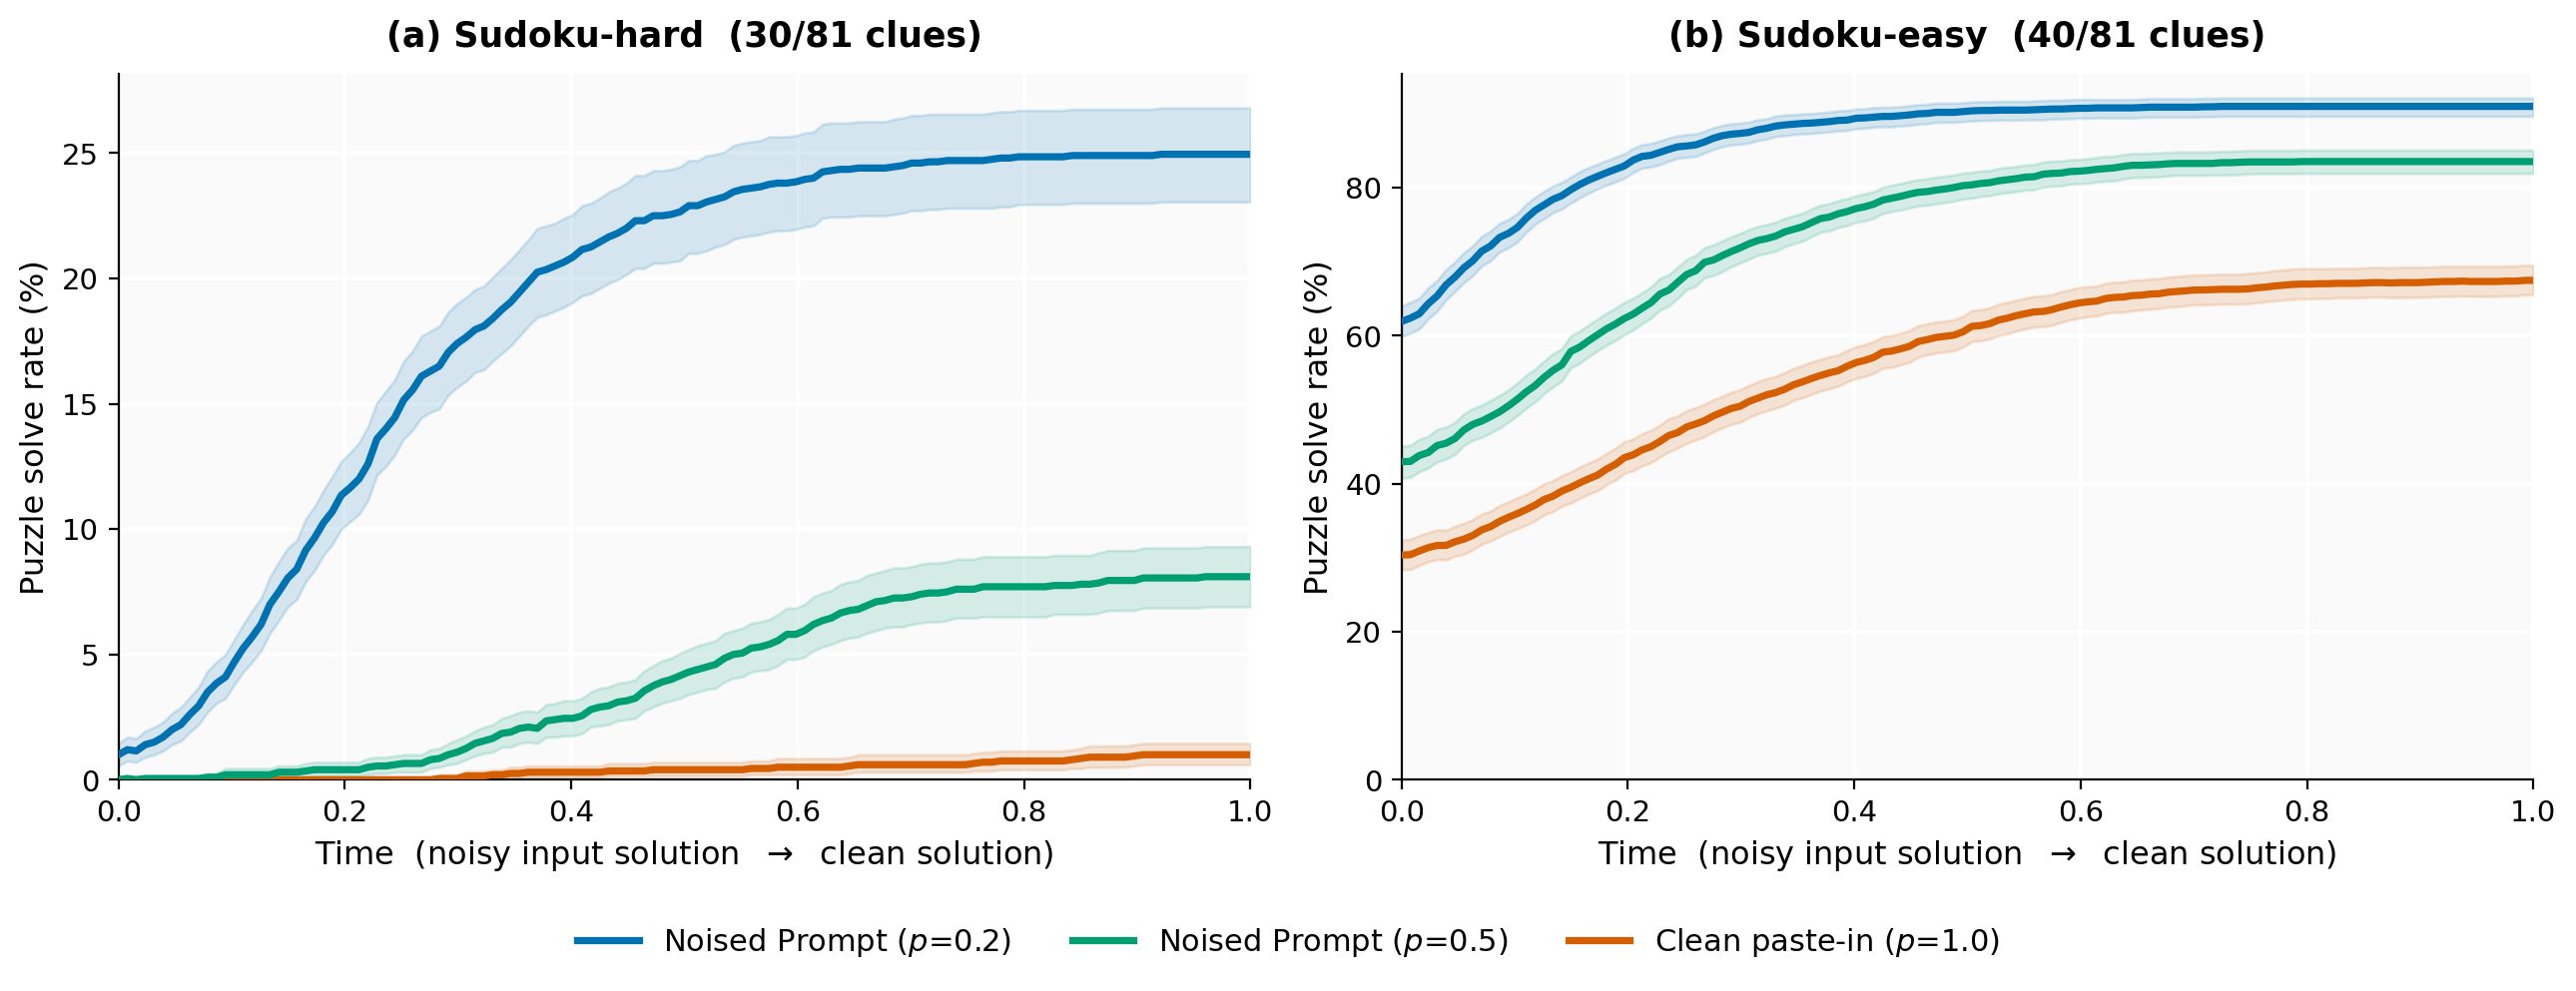
\includegraphics[width=0.95\linewidth]
  {figures/sudoku_solve_over_time_hard_easy.png}
\caption{
\textbf{Puzzle solve rate over the sampling trajectory.}
Puzzle (exact match) solve rate as a function of sampling time
(noisy input solution $\rightarrow$ clean solution), read from the model's $x_1$
prediction at each step. Means calculated over $2000$ held-out puzzles with a $128$-step
Euler sampler; shaded bands are $95\%$ bootstrap intervals over puzzles.
Across both difficulties the noised-prompt models ($p_\text{condclean}{=}0.2, 0.5$)
reach a substantially higher solve rate than the standard paste-in model
($p_\text{condclean}{=}1.0$) and also achieve their solve rate bound earlier in generation.
}
\label{fig:solverate}
  \end{figure}

\subsection{Setup}
\label{sec:setup}
Across all experiments the backbone is a DiT-style transformer \citep{peebles2023dit} with hidden size $512$,
$8$ blocks, $8$ attention heads, conditioning dimension $128$, and dropout $0.1$, trained with a
flow objective and $x_1$-prediction under a log-linear noise schedule. We optimize with
AdamW (learning rate $3\times10^{-4}$, $(\beta_1,\beta_2)=(0.9,0.999)$, no weight
decay), a constant schedule with $2{,}500$ warmup steps, gradient clipping at $1.0$,
bf16-mixed precision, and an EMA of $0.9999$. We use antithetic time sampling and a $t$-reparametrization
technique that adjusts for the vocabulary size \citep{flm}. 
Unless noted, we sample with a $128$-step Euler ancestral solver. The single swept variable is
$p_\text{condclean} \in \{0.2, 0.5, 1.0\}$ (and $0.0$ where noted); all other settings are held
fixed. Full hyperparameters are in Appendix~\ref{app:hyperparams}. All runs train on a single
NVIDIA L40S GPU. For Sudoku, the vocabulary designates token $0$ as
PAD, token $1$ an empty cell, and tokens $2$--$10$ as the digits $1$--$9$; for N-Queens,
token $0$ is PAD, token $1$ is an empty cell, and token $2$ is a queen.
Unlike prior work \citep{trm}, we train with no data augmentation.

\subsection{Metrics}
\label{sec:method-metrics}
We report two metrics. \textbf{Accuracy} is the fraction of generated boards that are valid
solutions to the puzzle (aggregated across all puzzles and samples). \textbf{Coverage} (N-Queens) is
a per puzzle statistic capturing the fraction of \emph{distinct} valid solutions
recovered across $k=20$ generated samples, all conditioned on the same input puzzle. This 
allows us to measure the diversity of the generations.

We report $95\%$ bootstrapping confidence intervals obtained by bootstrap resampling over the
evaluation puzzles ($10{,}000$ resamples; for N-Queens the resampling is over the $750$ input
boards, with per-board accuracy and coverage computed from that board's $k=20$ generations).

\subsection{Sudoku}
\label{sec:sudoku}
% TODO: Infill, full 9x9 board (length 81), difficulty easy, loss over board tokens.
%   Sweep p_condclean in {0.2, 0.5, 1.0}; data scales N=10,000 and N=1,000. 160k steps.
%   Eval on 2,000 puzzles. (experiment_log.md Runs 1-2; June 16 entry.)
% TODO: Table -- Sudoku-easy accuracy vs p_condclean:
%   N=10k: 0.2 -> 86.6%, 0.5 -> 74.75%, 1.0 -> 56.05%  (0.0 -> 2.85%, optional)
%   N=1k : 0.2 -> 11.0%, 0.5 -> 9.9%, 1.0 -> 2.3%       (0.0 -> 0.5%, optional)
% TODO: Observation -- monotonic: more noising (lower p) -> higher accuracy; ordering
%   preserved across data scale despite large absolute drop at N=1k.
Sudoku is a constraint-satisfaction puzzle on a $9\times9$ grid and a common benchmark for
reasoning and generalization ~\citep{trm, gram}. We use it precisely to measure generalization:
to solve unseen puzzles a model cannot simply memorize a mapping from $x \to y$, 
it must implicitly learn and respect the constraints of the game.

We train on Sudoku in the in-place infill layout: a full $9\times9$ board flattened row-wise (length $81$), with the
loss taken over all board tokens. Puzzles are generated following ~\citet{hyperspherical_flows}, and
difficulty is controlled by the number of revealed clues---$40$ of $81$ cells given for
\emph{easy} and $30$ of $81$ for \emph{hard}. We sweep $p_\text{condclean}$ at two training-set
sizes, $N=10{,}000$ and $N=1{,}000$ puzzles, at batch size $32$ or $256$ (easy: $160$k steps; hard: $40$k
steps respectively), and evaluate accuracy on $2{,}000$ held-out puzzles with a $128$-step sampler
(Table~\ref{tab:sudoku}).

\begin{table}[t]
\centering
\caption{Sudoku infill accuracy (\%) on $2{,}000$ held-out puzzles vs.\ the conditioning clean
probability $p_\text{condclean}$, with $95\%$ bootstrap CIs ($10{,}000$ resamples) in brackets.
Easy gives $40/81$ clues, hard $30/81$. At $N{=}10{,}000$, lower $p$ (more heavily noised clues)
yields higher accuracy on both difficulties; at the data-starved $N{=}1{,}000$ scale the easy
ordering breaks down ($p{=}0.5$ best) and hard sits at the floor. $p{=}1.0$ is the standard
``paste-in'' setup; $p{=}0.0$ is fully unconditional.}
\label{tab:sudoku}
\begin{tabular}{lcccc}
\toprule
& \multicolumn{2}{c}{Easy ($40/81$ clues)} & \multicolumn{2}{c}{Hard ($30/81$ clues)} \\
\cmidrule(lr){2-3}\cmidrule(lr){4-5}
$p_\text{condclean}$ & $N=10{,}000$ & $N=1{,}000$ & $N=10{,}000$ & $N=1{,}000$ \\
\midrule
$0.0$ (uncond.) & $1.50$ & --- & $0.00$ & --- \\
 & {\scriptsize $[1.00,\,2.05]$} & {\scriptsize ---} & {\scriptsize $[0.00,\,0.00]$} & {\scriptsize ---} \\
$0.2$ & $\mathbf{87.55}$ & $1.55$ & $\mathbf{25.45}$ & $0.05$ \\
 & {\scriptsize $[86.10,\,89.00]$} & {\scriptsize $[1.05,\,2.10]$} & {\scriptsize $[23.55,\,27.35]$} & {\scriptsize $[0.00,\,0.15]$} \\
$0.5$ & $76.60$ & $\mathbf{14.40}$ & $7.70$ & $\mathbf{0.10}$ \\
 & {\scriptsize $[74.75,\,78.45]$} & {\scriptsize $[12.85,\,16.00]$} & {\scriptsize $[6.55,\,8.90]$} & {\scriptsize $[0.00,\,0.25]$} \\
$1.0$ (paste-in) & $51.45$ & $2.70$ & $1.25$ & $0.00$ \\
 & {\scriptsize $[49.30,\,53.60]$} & {\scriptsize $[2.00,\,3.45]$} & {\scriptsize $[0.80,\,1.75]$} & {\scriptsize $[0.00,\,0.00]$} \\
\bottomrule
\end{tabular}
\end{table}

The default setup of pasting-in clean conditioning tokens during training performs 
notably worse than our method of noising conditioning tokens across all Sudoku settings. 
On Sudoku easy, $p{=}0.2$ reaches $87.55\%$ versus
$51.45\%$ for the standard paste-in setup; on hard, $25.45\%$ versus $1.25\%$. 
Under the data-limited regime $N=1{,}000$, $p{=}0.5$ performs best; 
the default paste-in strategy and $p{=}0.2$ perform similarly, with no statistically significant
difference in performance. 

The fully-unconditional setup ($p=0.0$) exhibits poor generation, demonstrating that the model still needs to see
some conditioning tokens as clean.


\subsection{N-Queens}
\label{sec:nqueens}
% TODO: Infill on n*n board, tokens {0=pad,1=empty,2=queen}; sweep p_condclean {0.2,0.5,1.0}.
%   Last checkpoint, 750 puzzles x 20 samples. N=8 (length 64) and N=10 (length 100).
%   (experiment_log.md Runs 3-4; June 18-19 entries.)
% TODO: Table -- accuracy & coverage vs p_condclean:
%   N=8  (750x20): 0.2 -> 99.24/97.31; 0.5 -> 98.75/91.41; 1.0 -> 97.67/88.07
%   N=10 (750x20): 0.2 -> 94.66/80.01; 0.5 -> 57.42/71.05; 1.0 -> 64.56/64.03
% TODO: Observation -- coverage monotonic across BOTH n; p=0.2 dominates. Flag the N=10
%   ACCURACY non-monotonicity (p=0.5 below p=1.0): robust claim is coverage ordering +
%   dominance of heavy noising, not strict accuracy monotonicity. Possibly single-seed noise
%   -- note variance caveat (notes Run 4).

N-Queens is a puzzle where $n$ mutually non-attacking queens must be placed on a 
$n\times n$ board and is
likewise used to evaluate reasoning and generalization of models~\citep{gram}. In addition to being 
combinatorial in nature,
N-Queens admits multiple valid solutions for a given starting board. This allows us to measure the
diversity of the generated solutions. Following GRAM~\citep{gram}, we track coverage of possible
solutions and report the number of unique solutions generated out of the total number of possible solutions corresponding to
that board. We evaluate on held out initial board states and generate 20 samples per input
board. 

We consider two scales, $n=8$ (length $64$) and $n=10$ (length $100$). We subsample the data
such that puzzles of varying difficulty (as defined by the number of initial queens) are equal
in number. For $n=8$ this yields $1{,}758$ training / $174$ validation puzzles; for
$n=10$ we have $5{,}717$ training / $557$ validation puzzles. Training and evaluation splits are
disjoint by input board. We train at global batch size $256$ for $100$k
steps and evaluate the final checkpoint on $750$ held-out puzzles with $20$ generations each
(Table~\ref{tab:nqueens}).

\begin{table}[t]
\centering
\caption{N-Queens infill accuracy and coverage (\%), final checkpoint, $750$ puzzles
$\times\,20$ samples, with $95\%$ bootstrap CIs ($10{,}000$ resamples over input boards) in
brackets. Both accuracy and coverage are monotonic in $p_\text{condclean}$ at both scales, and
$p{=}0.2$ dominates throughout.}
\label{tab:nqueens}
\begin{tabular}{lcccc}
\toprule
& \multicolumn{2}{c}{$n=8$ (length 64)} & \multicolumn{2}{c}{$n=10$ (length 100)} \\
\cmidrule(lr){2-3}\cmidrule(lr){4-5}
$p_\text{condclean}$ & Accuracy & Coverage & Accuracy & Coverage \\
\midrule
$0.2$ & $\mathbf{99.16}$ & $\mathbf{92.97}$ & $\mathbf{97.90}$ & $\mathbf{73.93}$ \\
 & {\scriptsize $[98.61,\,99.60]$} & {\scriptsize $[91.75,\,94.16]$} & {\scriptsize $[97.37,\,98.37]$} & {\scriptsize $[72.54,\,75.36]$} \\
$0.5$ & $98.97$ & $90.88$ & $94.23$ & $60.68$ \\
 & {\scriptsize $[98.48,\,99.39]$} & {\scriptsize $[89.51,\,92.22]$} & {\scriptsize $[93.25,\,95.14]$} & {\scriptsize $[59.12,\,62.28]$} \\
$1.0$ (paste-in) & $97.67$ & $88.07$ & $84.80$ & $49.89$ \\
 & {\scriptsize $[96.73,\,98.51]$} & {\scriptsize $[86.46,\,89.63]$} & {\scriptsize $[83.09,\,86.42]$} & {\scriptsize $[48.21,\,51.56]$} \\
\bottomrule
\end{tabular}
\end{table}

At $n=8$ accuracy is high throughout; whereas at $n=10$ the noised conditioning 
tokens at ($p=0.2$) performs substantially better over the default paste-in setup.

Coverage is a more salient metric: for both $n=8$ and $n=10$, training on just clean conditioning 
tokens leads to lower diversity of generations, prominently demonstrated at $n=10$ ($49.89$ vs $73.93\%$)

The general trend of our experiments yield that more frequent noising of the conditioning tokens
lead to both higher accuracy and higher coverage.  

\subsection{Ablations}
\label{sec:ablations}
We consider the following three ablations to illustrate the design choice of our noising scheme:
(i) whether the conditioning tokens are noised to the same time as the response or to an independent time;
(ii) whether the loss is computed over the full sequence or only the response tokens; and (iii) the
whether the model needs to see clean conditioning tokens at all (fully unconditional training).
All numbers are calculated with $95\%$ bootstrap CIs
($10{,}000$ resamples; Sudoku $n{=}2{,}000$, N-Queens $750$ input boards).

\paragraph{Separate conditioning time.}
The current objective noises conditioning tokens to the same sampled noise level (parameterized by time) as the response tokens.
We consider drawing an independent time $t' \sim \mathcal{U}(0,1)$ for the conditioning tokens, so
the conditioning and response are corrupted to decoupled noise levels. 

On Sudoku-easy ($N{=}10{,}000$, $p_\text{condclean}{=}1.0$) it reaches
$90.45\%$, above the best single-time setting in Table~\ref{tab:sudoku} ($87.55\%$ at $p{=}0.2$),
while on Sudoku-hard it performs worse at $21.80\%$. On N-Queens it does not beat frequent same time
noising: $n{=}8$ reaches $97.31\%$ accuracy / $89.52\%$ coverage and $n{=}10$ reaches $87.41\%$ /
$51.40\%$, below the $p{=}0.2$ (Table~\ref{tab:nqueens}).

\paragraph{Loss calculated on full sequence vs response only.}
We ablate a response-tokens only loss objective that excludes the conditioning tokens predictions,
sweeping $p_\text{condclean}$ on Sudoku-easy ($N{=}10{,}000$). By incorporating only the response 
tokens in the loss, the model performs worse, validating our position 
that a full sequence objective is a more efficient and effective training objective. 

\paragraph{Only noised conditioning tokens ($p_\text{condclean}{=}0$).}
With conditioning tokens always noised, the model learns the unconditional distribution 
but is unable to utilize the given clean conditioning information at inference time. On Sudoku hard
 ($N{=}10{,}000$) accuracy collapses to $0\%$; and on Sudoku easy ($N{=}10{,}000$) accuracy is $1.50\%$.
This confirms that some exposure to clean conditioning tokens is necessary.

\begin{table}[t]
\centering
\caption{Ablations (accuracy / coverage \%, with $95\%$ bootstrap CIs). \emph{Top:} separate
conditioning-time variant (independent clue time $t'$). \emph{Middle:} response-only loss
region on Sudoku-easy ($N{=}10{,}000$), swept over $p_\text{condclean}$. \emph{Bottom:}
unconditional floor on Sudoku-easy and Sudoku-hard ($N{=}10{,}000$); the Sudoku-easy value is the
$p{=}0.0$ row of Table~\ref{tab:sudoku}. No N-Queens runs for the loss-region and unconditional
ablations.}
\label{tab:ablations}
\begin{tabular}{llcc}
\toprule
Ablation & Setting & Accuracy & Coverage \\
\midrule
\multirow{4}{*}{Separate cond.\ time}
 & Sudoku easy  & $90.45$ {\scriptsize $[89.15,91.70]$} & --- \\
 & Sudoku hard  & $21.80$ {\scriptsize $[20.00,23.60]$} & --- \\
 & N-Queens $n{=}8$ & $97.31$ {\scriptsize $[96.32,98.18]$} & $89.52$ {\scriptsize $[88.06,91.00]$} \\
 & N-Queens $n{=}10$ & $87.41$ {\scriptsize $[85.83,88.91]$} & $51.40$ {\scriptsize $[49.74,53.10]$} \\
\midrule
\multirow{4}{*}{\shortstack[l]{Response-only loss\\(Sudoku easy)}}
 & $p{=}0.0$ & $2.60$ {\scriptsize $[1.95,3.30]$} & --- \\
 & $p{=}0.2$ & $83.80$ {\scriptsize $[82.20,85.40]$} & --- \\
 & $p{=}0.5$ & $46.50$ {\scriptsize $[44.35,48.65]$} & --- \\
 & $p{=}1.0$ & $36.95$ {\scriptsize $[34.90,39.15]$} & --- \\
\midrule
\multirow{2}{*}{Unconditional ($p{=}0$)}
 & Sudoku easy & $1.50$ {\scriptsize $[1.00,2.05]$} & --- \\
 & Sudoku hard & $0.00$ {\scriptsize $[0.00,0.00]$} & --- \\
\bottomrule
\end{tabular}
\end{table}

\section{Analysis and Discussion}
\label{sec:analysis}
\paragraph{Why does noising the conditioning help?}
We posit views consistent with the results above. First, noising the conditioning tokens 
leads to a wider set of training inputs and also makes use of the conditioning token predictions 
in the loss. Second, by decreasing the amount of signal in conditioning tokens, the model becomes
less reliant on predicting responses mainly based on the condition, leading to a greater 
variety of generations, as exhibited by the mode coverage results (always-clean training ($p=1$) collapses toward fewer solutions).
Finally, incorporating both noisy conditional tokens and non-noisy conditioning tokens can be 
seen as curriculum learning: $p<1$ mixes an easier prediction task (given fully clean condition signal)
with a harder (given noised conditioning signal) prediction task. 

\paragraph{Relation to classifier-free guidance.}
Because $p$ interpolates between a conditional-only ($p=1$) and unconditional-only ($p=0$) objective,
our scheme can be viewed as a continuous generalization of classifier-free guidance training. 
Currently we only consider fully clean conditioning tokens at inference time; 
combining predictions under fully clean conditioning tokens and partially noised conditioning 
tokens during sampling may be a natural next direction. 

\paragraph{Limitations.}
We train on relatively small models and trained on small datasets. Future work
would include evaluating on much larger models and consider scaling behavior.
Our bootstrap CIs control for evaluation sampling variance, but not for
training seed variance. We evaluate on combinatorial reasoning tasks such as Sudoku and N-Queens. 
While we have not run sufficient experiments on natural language reasoning datasets due to compute
restrictions, this is a direction we hope to see.   

\section{Conclusion}
\label{sec:conclusion}
We revisited an accepted default practice of keeping conditioning tokens clean during training
of continuous diffusion language models and showed that simply noising the conditioning tokens
as well during training improves conditional generation quality and diversity. The method is a trivial engineering change to the training objective and
can be seen as a continuous generalization of classifier-free guidance training. 
Future work includes scaling analysis with larger models, using language dataset benchmarks,
and incorporating noised conditioning tokens during sampling-time. 

\bibliography{references}
\bibliographystyle{colm2026_conference}

\appendix
\section{Full Hyperparameters}
\label{app:hyperparams}
Table~\ref{tab:hparams} lists the shared training configuration (N-Queens Run; Sudoku differs only
in board length $81$, batch size $32$, and $160$k training steps).

\begin{table}[h]
\centering
\caption{Shared hyperparameters}
\label{tab:hparams}
\begin{tabular}{lll}
\toprule
Group & Setting & Value \\
\midrule
Model & hidden size / blocks / heads & $512$ / $8$ / $8$ \\
      & cond.\ dim / dropout & $128$ / $0.1$ \\
      & board length & $81$ (Sudoku), $64$/$100$ (N-Queens $n{=}8$/$10$) \\
Algorithm & parameterization / pred.\ type & mean / $x_1$ \\
          & loss type & flow \\
          & diffusion forcing & true \\
          & $p_\text{condclean}$ & $\{0.2,0.5,1.0\}$ (swept) \\
Noise & type / eps & log-linear / $0$ \\
Training & max steps & $100{,}001$ (N-Queens), $160$k (Sudoku) \\
         & global batch size & $256$ (N-Queens), $32$ (Sudoku) \\
         & precision / EMA & bf16-mixed / $0.9999$ \\
         & grad clip & $1.0$ \\
         & $t$-curriculum & $0.0\to1.0$ over $100$k steps \\
Optimizer & class & AdamW \\
          & lr / $(\beta_1,\beta_2)$ / wd & $3\!\times\!10^{-4}$ / $(0.9,0.999)$ / $0$ \\
          & warmup & $2{,}500$ steps (constant after) \\
Sampling & predictor / solver & ancestral / Euler \\
         & steps / temperature / nucleus & $128$ / $1.0$ / $1.0$ \\
Hardware & accelerator / GPU & cuda, 1 device / NVIDIA L40S \\
\bottomrule
\end{tabular}
\end{table}

\end{document}
